\documentclass[11pt,oneside,spanish,a4paper]{article}
\usepackage[utf8]{inputenc}
\usepackage[spanish]{babel}
\usepackage[a4paper]{geometry}
\usepackage{graphicx}
\usepackage{fancyhdr}
\usepackage[hyphenbreaks]{breakurl}
\usepackage[hyphens]{url}
\usepackage{hyperref}
\usepackage{listings}
\usepackage{lstlinebgrd}
\usepackage{xcolor}
\usepackage{multicol}
\usepackage{pdfpages}
\usepackage{amssymb}
\usepackage{mathtools}
\usepackage{lineno}
\usepackage{caption}
\usepackage{subcaption}

%%%%%%%%%%%%%%%%%%%%
% Nuevos comandos  %
%%%%%%%%%%%%%%%%%%%%
\newcommand{\HRule}{\rule{\linewidth}{0.5mm}}

\hypersetup{
    pdfcreator={pdfLaTeX},   % creator of the document
    colorlinks=true,       % false: boxed links; true: coloblue links
    linkcolor=blue,          % color of internal links (change box color with linkbordercolor)
    citecolor=blue,        % color of links to bibliography
    filecolor=blue,      % color of file links
    urlcolor=blue           % color of external links
}

\pagestyle{fancy}
\addtolength{\textheight}{2cm}
%\addtolength{\voffset}{-1cm}
%\addtolength{\textwidth}{1cm}

\definecolor{light-gray}{gray}{0.9}

\lstset{
  basicstyle=\ttfamily\color{red},%\footnotesize,%\scriptsize,
  language=tcl,
  breaklines=true,
  otherkeywords={+++},
  numbers=left,
  numberstyle=\scriptsize\color{black}
}

\renewcommand{\lstlistingname}{Código}

\lstset{literate=
  {á}{{\'a}}1 {é}{{\'e}}1 {í}{{\'i}}1 {ó}{{\'o}}1 {ú}{{\'u}}1
  {Á}{{\'A}}1 {É}{{\'E}}1 {Í}{{\'I}}1 {Ó}{{\'O}}1 {Ú}{{\'U}}1
  {à}{{\`a}}1 {è}{{\'e}}1 {ì}{{\`i}}1 {ò}{{\`o}}1 {ù}{{\`u}}1
  {À}{{\`A}}1 {È}{{\'E}}1 {Ì}{{\`I}}1 {Ò}{{\`O}}1 {Ù}{{\`U}}1
  {ä}{{\"a}}1 {ë}{{\"e}}1 {ï}{{\"i}}1 {ö}{{\"o}}1 {ü}{{\"u}}1
  {Ä}{{\"A}}1 {Ë}{{\"E}}1 {Ï}{{\"I}}1 {Ö}{{\"O}}1 {Ü}{{\"U}}1
  {â}{{\^a}}1 {ê}{{\^e}}1 {î}{{\^i}}1 {ô}{{\^o}}1 {û}{{\^u}}1
  {Â}{{\^A}}1 {Ê}{{\^E}}1 {Î}{{\^I}}1 {Ô}{{\^O}}1 {Û}{{\^U}}1
  {œ}{{\oe}}1 {Œ}{{\OE}}1 {æ}{{\ae}}1 {Æ}{{\AE}}1 {ß}{{\ss}}1
  {ç}{{\c c}}1 {Ç}{{\c C}}1 {ø}{{\o}}1 {å}{{\r a}}1 {Å}{{\r A}}1
  {€}{{\EUR}}1 {£}{{\pounds}}1 {"}{{``}}1
}

\begin{document}

%%%%%%%%%%%%%%%%%%%%%%%%%
% Carátula del informe  %
%%%%%%%%%%%%%%%%%%%%%%%%%

\begin{titlepage}
\begin{center}

\textsc{\LARGE Instituto Universitario Aeronáutico}\\[0.5cm]
\textsc{\LARGE Especialización en Sistemas Embebidos}\\[2cm]


\includegraphics[width=0.2\textwidth]{img/logo_f_blanco}~\\[2cm]

\textsc{\Large Entornos Inalámbricos}\\[0.5cm]

\HRule \\[0.4cm]
{ \huge \bfseries Trabajos Prácticos \\[0.4cm] }

\HRule \\[1.5cm]

% Author and supervisor
\begin{minipage}{0.4\textwidth}
\begin{flushleft} \large
\emph{Alumno:}\\
Luis Alberto \textsc{Guanuco}\\
Santiago Nicolás \textsc{Nolasco}\\
Sebastian \textsc{Agüero}\\
Franco \textsc{Bocalon}
\end{flushleft}
\end{minipage}
\begin{minipage}{0.4\textwidth}
\begin{flushright} \large
\emph{Docentes:} \\
Víctor \textsc{Frison}\\
Julio \textsc{Echevarría}\\
José \textsc{Ducloux}
\end{flushright}
\end{minipage}
\vfill
{\large Septiembre 2016}

\end{center}
\end{titlepage}

%\lhead{Luis A. Guanuco}
%\chead{\includegraphics[width=0.02\textwidth]{images/logoUTN}}
%\rhead{Arquitectura Embebidas y Proceso de Tiempo Real}
\section{Introducción}
\label{sec:intro}

Se realizarán ejercitaciones sobre plataformas XBee con el objetivo
de entender los \emph{Entornos Inalámbricos}. Se trabajará con los
modos \emph{AT} y \emph{API} a fin de comprar las ventajas y
desventajas de estos. Estos ejemplos prácticos servirán, además,
alcanzar la resolución del \emph{Trabajo Final}.

\subsection{Módulos XBee S2C}
\label{sec:xbee-mod}

Para el establecimiento de una red basado en los estándares 802.15.4
se plantea como requisito la disponibilidad de módulos que implementen
dicho estándar. En nuestro caso se utilizarán los módulos \emph{XBee
  S2C}\footnote{\burl{http://www.digi.com/support/productdetail?pid=4838}}. Las
principales características de estos dispositivos son:
\begin{itemize}
\item Velocidades de datos
  \begin{itemize}
  \item RF 250 Kbps
  \item Comunicación serial hasta 1 Mbps
  \end{itemize}
\item Alcances
  \begin{itemize}
  \item \textsl{Indoor} 60 metros
  \item \textsl{Outdoor} 1200 metros
  \end{itemize}
\item Potencia de transmisión 3.1 mW (+5 dBm). En modo \textsl{Boost}
  6.3 mW (+8 dBm)
\item Sensibilidad de recepción -100 dBm. EN modo \textsl{Boost} -102
  dBm
\item Banda de frecuencia 2.4 GHz (16 canales)
\item 15 puertos digitales I/O (4 entradas analógicas)
\item Alimentación 2.1V a 3.6V. Consumos:
  \begin{itemize}
  \item En la transmisión 33 mA @ 3.3 VDC. En modo \textsl{Boost}45 mA
  \item En la recepción 28 mA @ 3.3 VDC. En modo \textsl{Boost} 31 mA
  \end{itemize}
\end{itemize}

Los puntos anteriores solo describen las principales características
de los módulos XBee 2SC. Para conocer más en detalle se puede acceder
a la hoja de datos disponible en el sitio web del fabricante
\cite{s2c-ds}.

\subsection{Plataformas adicionales}
\label{sec:plat}

Se utilizará \textsl{hardware} adicional que permita establecer la
comunicación de los módulos XBee con una computadora. Sí bien el
Laboratorio de Sistemas embebidos pone a disposición las plataformas
XBoard\footnote{\burl{http://www.cika.com/soporte/Information/Digi-RF/XBee/}}
se necesita adaptar la comunicación serial del módulo XBee con la la
computadora mediante una puerto USB. Para esto se desarrolló la placa
\emph{XBee-MCP Adapter} (Figura \ref{fig:xb-mcp-adap}). Sobre esta
placa se montarán dos módulos, una es el módulo XBee y el otro es la
placa \emph{MCP2200 Breakout
  Module}\footnote{\burl{http://www.microchip.com/DevelopmentTools/ProductDetails.aspx?PartNO=adm00393}}. Este
último proporciona una comunicación serial USB-UART. 
Además se agregaron dos LEDs conectados a los puertos
\texttt{AD1/DIO1} y \texttt{AD2/DIO2}. Opcionalmente se puede conectar
un potenciómetro al conector \texttt{K1} que se encuentra mapeado al
puerto analógico de la XBee, \texttt{AD0/DIO0}.

\begin{figure}[h]
  \centering
  \includegraphics{img/xb-mcp-adapter}
  \caption{Placa XBee-MCP Adapter.}
  \label{fig:xb-mcp-adap}
\end{figure}

La Xboard, anteriormente mencionada, es una plataforma desarrollada
por la empresa Cika Electrónica SRL. La XBoard permite interconectar
los módulos XBee con dispositivos externos \cite{xboard}. En la Figura
\ref{fig:xboard} se presenta una vista superior de la XBoard. Se puede
ver que esta placa tiene un conector hembra con las señales de
comunicación serial, niveles de tensión y otras más. Para conectar la
XBoard a una computadora se utiliza la placa MCP2200 Breakout
Module. Al no requerir componentes externos, se utilizan simplemente
cables que realicen la interconexión de las señales de comunicación
serial.

\begin{figure}[h]
  \centering
  \includegraphics[width=.6\textwidth]{img/xboard}
  \caption{Placa XBoard.}
  \label{fig:xboard}
\end{figure}

Todas las características y configuraciones de las diferentes
plataformas comerciales  se encuentran en la bibliografía referenciada
al final de este documento. 

Se desarrollarán tres tipos de ejercitaciones. La primera sobre los
alcances de RF que proporcionan estos dispositivos. La segunda parte
sobre el manejo de los módulos en modo AT. Y por último se trabajará
en modo API con los módulos sobre una red ZigBee completa. Se
documentarán todos las implementaciones y por último se presentará una
conclusión sobre lo hecho.

\section[Enlace y propagación]{C\'alculo de enlace y modelos de propagaci\'on}
\label{S:1}

El dise\~no de un radioenlace implica toda una serie de c\'alculos que pueden resultar sencillos o complicados, dependiendo de las caract\'eristicas del sistema y del tipo de problema al que nos enfrentemos.

Es por ello que podemos dividir la propagaci\'on de la se\~nal de acuerdo al entorno donde esta viaje: 

\begin{itemize}
\item Espacios abiertos 
\item Entornos cerrados
\end{itemize}


\subsection[Distancias]{Distancia m\'axima en espacios abiertos}

 La comunicaci\'on ``outdoor'' en este problema se asume en un entorno de propagaci\'on libre, donde no existen p\'erdidas atmosf\'ericas, de polarizaci\'on y de desadaptaci\'on de impedancias, es decir, operamos en regiones descubiertas. 
 
\begin{figure}[h]
	%\DeclareGraphicsExtensions{.pdf,.png,.jpg,.ppm}
	\centering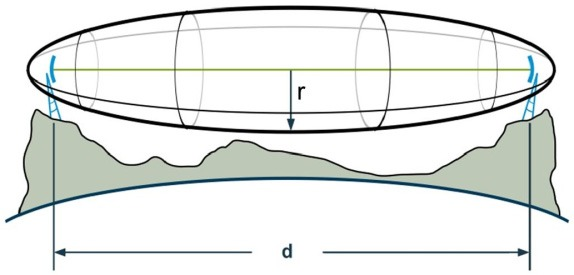
\includegraphics[width=0.8\linewidth]{img/Image}
	\caption{Primer zona de Fresnel}
\end{figure}

\begin{table}[h]
	\centering
	\begin{tabular}{l l l}
		\hline
		\textbf{Modo de funcionamiento} & \textbf{Normal} & \textbf{Boost}\\
		\hline
		Potencia de Tx & +5dBm(3.1mW) & +8dBm(6.3mW) \\
		Sensibilidad de Rx & -100dBm & -102dBm\\
		\hline
	\end{tabular}
	\caption{Technical review Xbee S2C}
\end{table}
Para los c\'alculos siguientes se tomar\'an los datos de funcionamiento en modo ``Normal''.

Partiendo de la ecuaci\'on de Friis\cite{bilb:Friis}

%\begin{equation}
%\label{Ecuaci\'on de Friis}

%Pr = \frac{Pt Gt Gr \lambda ^{2}}{(4\pi R)^2}

%\end{equation}

\begin{equation*}
\label{Ec:Friis}
Pr = \frac{Pt Gt Gr \lambda ^{2}}{(4\pi d)^2}
\end{equation*}
Siendo Pr (Potencia recibida), Pt(Potencia transmitida), Gt(Ganancia de antena tx), Gr(Ganancia de antena rx), $\lambda$(longitud de onda) y d(distancia radial entre antenas).

Podemos despejar la atenuaci\'on de espacio libre, tambi\'en conocida como p\'erdida de trayectoria\cite{bilb:Free}.
\begin{equation*}
\label{Ec:perdida}
P_{Loss}[dB] = 94.4 dB + 20 \log_{10}d [Km] + 20 \log_{10}f [GHz] - Gt[dBi] - Gr[dBi]
\end{equation*}
Y de esta despejar la m\'axima distancia(adicionamos -5dB de atenuaci\'on, por margen)
\begin{equation*}
\label{Ec:distancia}
d[Km] = 10^{\frac{P_{Loss} + Gt + Gr - 20 \log_{10}f - 92.4dB -5dB}{20}}
\end{equation*}
$P_{Loss}=Gt[dBm] - Gr[dBm] = +5dBm - (-100dBm) = 105dBm$
$f = 2.4 [GHz]$
Las ganancias Gr[dBi] y Gr[dBi] se toman como valor cero por ser antenas omnidireccionales.
\begin{equation*}
\label{Ec:distancia1}
d[Km] = 10^{\frac{105 dBm - 20 \log_{10}2.4 - 92.4dB-5dB}{20}} = 0.999 [Km] =999m
\end{equation*}	
Con la m\'axima distancia $d$ del radioenlace, calculamos la altura $r$ de las antenas. Para ello nos valemos de las f\'ormulas del primer elipsoide de Fresnel, esto es determinando la zona libre de obstaculos\cite{bilb:Fresnel}.
\begin{equation*}
\label{Ec:fresnel}
r = F1(m) = 17.32 \sqrt{\frac{(d[Km]/2)^2}{d[Km]f[GHz]}} = 17.32 \sqrt{\frac{(0.99Km/2)^2}{0.99Km2.4GHz}} = 7.28m
\end{equation*}	

Por lo tanto la altura de las antenas, es decir para establecer una comunicaci\'on punto a punto a distancia m\'axima $d=999m$ entre 2 XBee es de $r=7.28m$ en la zona libre de obstaculos.Adem\'as este es un valor muy cercano al valor$d=1200m$ dado por la hoka de datos de la XBee.

\subsection{Distancia m\'axima en entornos cerrados}

La propagaci\'on ``indoor'' difiere respectos a los sistemas ``outdoor''. Para asegurar una eficiente comunicaci\'on interior, la ITU a llevado una serie de propuestas para el caso de comunicaciones punto a punto. Debido a que en una comunicaci\'on en entornos cerrados esta muy influenciada por la geometr\'ia del lugar y los objetos en ella. Tanto estos objetos y la construcci\'on de la misma, ocasionan p\'erdidas por reflexiones, dispersi\'on y absorci\'on de las se\~nales RF.  

\begin{figure}[h]
	\centering\includegraphics[width=0.6\linewidth]{img/xbee-ejemplo.png}
	\caption{Comunicaci\'on indoor}
\end{figure}

\subsubsection{C\'alculo Planta alta}
Para el c\'alculo de m\'axima distancia, como lo indica la figura. Nos valdremos de la f\'ormula de ``path loss''\cite[Pág.4]{bilb:PathLoss}
\begin{equation*}
\label{eq:pathLoss}
L_{Loss}[dB] = L_{do}[dB] + N \log_{10}d/do + Lf_{n}[dB]
\end{equation*}
Donde $N$(Coef. de p\'erdida), $f$(Frecuencia en Mhz),$d$(Distancia entre base y terminal), $L_{do}$(P\'erdida a do), $L_{f}$(Atenuaci\'on trav\'es del piso), $d0$(distancia de ref=1m) y $n$(nro de pisos entre terminal y base).
En nuestro caso particular al igual que en el caso anterior, calculamos la m\'axima atenuaci\'on:
$L_{Loss}= Gt - Gr = +5dBm - (-100dBm) = 105dBm$
$N=28$ Por dato de tabla \cite[Pág 4-5]{bilb:PathLoss}(Espacio residencial a 2.4GHz).
$L_{do} = 20 \log_{10}f[MHz] - 28 = 39.6dB$
$Lf_{n} = 0$ Por ser un mismo piso.
Despejando d, incluyendo una atenuaci\'on adicional de 10dB por la cantidad de objetos que puedan influir en la comunicaci\'on.
\begin{equation*}
\label{eq:calculod}
d[m] = 10 ^{\frac{L_{Loss}[dB] - L_{do}[dB] - L_{f}-10dB[dB]}{N}} 
d[m] = 10 ^{\frac{105dBm - 39.6dB - 0dB - 10dB}{28}} = 95.18m
\end{equation*}
Entonces en un piso la distancia m\'axima de transmisi\'on es $d=95.18m$

\subsubsection{C\'alculo de comunicaci\'on entre Planta alta y baja}
En este caso la m\'axima distancia $d$, ser\'a influenciada por la atenuaci\'on del piso, como separaci''on de los dos ambientes. Por lo tanto $L_{f}[dB]=5$ dado por el cuadro, adicionamos una atenuaci\'on de 10dB . La distancia m\'axima ser\'a.
\begin{equation*}
\label{eq:calculod}
d[m] = 10 ^{\frac{L_{Loss}[dB] - L_{do}[dB] - L_{f}[dB]}{N}} 
d[m] = 10 ^{\frac{105dBm - 39.6dB - 5dB -10dB}{28}} = 63.09m
\end{equation*}
Se puede notar aqu\'i, que el valor de $d$ distancia m\'axima es reducido por esta atenuaci\'on. Siendo el valor de $d=63.09m$ para comunicaciones entre dos pisos. Lo que es comparable al $d=60m$ dado por la hoja de datos.

\section{Ejercitación en modo AT}
\label{sec:AT}

El set de comandos AT, también conocidos como set de comandos Hayes,
fue originalmente desarrollado para usar con los modem de Hayes en la
década de 1980. Muchos modems modernos todavía utilizan este
estándar. EL término \emph{comando AT}  viene de usar los caracteres
ASCII para notificar al \textsl{host}  que un le sigue un comando. 

En el caso de los módulos XBee desarrollados por Digi, implementa un
set de comandos propieratrios para interactuar con los módulos de
Digi a través de una comunicación serial. Basado en el set de comandos
AT, Digi usa los caracteres \texttt{AT} antes de cada comando enviado
al modem. Un ejemplo de un comando utilizado por el radio Digi XBee
podría ser \texttt{ATCH}. Este comando es usado para leer o setear el
canal que un radio XBeee es configurado\cite{at-cmds}.

\subsection{Configuración de puertos GPIO}
\label{sec:config-at}

La configuración de los diferentes canales de propósitos generales se
puede realizar utilizando el software XCTU en modo gráfico pero el
objetivo es realizarlo mediante el set de comandos AT. 

\subsubsection{Comando ATIS}
\label{sec:atis}

El comando \texttt{ATIS} fuerza la lectura de todos los canales
habilitados. Analógicos como digitales. En nuestro caso tenemos la
siguiente salida a la petición.

\begin{lstlisting}[emph={+++,ATIS}, emphstyle={\color{blue}}]
+++
OK
ATIS
01
0006
01
0000
0219
\end{lstlisting}

La respuesta que entrega el módulo comienza en la línea \textbf{4}
hasta la \textbf{8}. El primer byte \texttt{01} es la cantidad de
muestra recibidas. En la línea \textbf{5} se tiene configuración de
los canales digitales y la línea \textbf{6} canales analógicos. Para
entender se debe analizar a nivel de bits cada una de las
respuestas. Recuerde que los valores representados están en
hexadecimal. En el primer se tiene $0006_{HEX} =
000000000000110_{BIN}$ por lo los canales \texttt{DIO1} y
\texttt{DIO2} se encuentran habilitados y configurados como salidas
digitales. Mientras que para los canales analógicos tenemos
$01_{HEX} = 0001_{BIN}$ solo el puerto \texttt{AD0} habilitado. Para
terminar el análisis de la respuesta al comando \texttt{ATIS}, las
líneas \textbf{7} y \textbf{8} son el estado de los canales
digitales y analógicos respectivamente. Como se mencionó
anteriormente, puede visualizarse la configuración de los canales de
I/O en forma gráfica desde el software XCTU. En la Figura
\ref{fig:xctu-setup} se puede ver la misma información que
proporciona el comando \texttt{ATIS}.

\begin{figure}[h]
  \centering
  \includegraphics[width=.8\textwidth]{img/xctu-atis}
  \caption{Configuración de los GPIO en modo gráfico.}
  \label{fig:xctu-setup}
\end{figure}

Para dar comienzo con la ejercitación pedida por los docentes, se
deshabilitarán todos los canales de forma tal que el módulo quede sin
ningún GPIO en uso. Sí la configuración es tal como la descrita
anteriormente, se deben aplicar los comandos siguientes.

\noindent\begin{minipage}{.25\textwidth}
\begin{lstlisting}[emph={+++,ATIS,ATD00,ATD10,ATD20,ATWR,ATAC}, emphstyle={\color{blue}}]
+++OK
ATD00
OK
ATD10
OK
ATD20
OK
ATAC
OK
ATWR
OK
ATIS
ERROR
\end{lstlisting}
\end{minipage} \hfill
\begin{minipage}{.70\textwidth}
Para deshabilitar un canal digital/analógico se debe simplemente pasar
como último argumento el valor \texttt{0}. Esto se aplica a los
canales \texttt{DIO0}, \texttt{DIO1} y \texttt{DIO2}. Los comandos que
le siguen son para aplicar los cambios y liberar los \textsl{buffers}
(\texttt{ATAC}) y  escribir la
memoria no-volatil del módulo (\texttt{ATWR}). Al finalizar los
cambios se envía el comando \texttt{ATIS} y se tiene como respuesta
\texttt{ERROR} esto no se debe a un problema de comunicación sino que
al no existir ningún canal habilitado, no puede ofrecer información
alguna. 
\end{minipage}

A continuación se presentan diferentes configuraciones sobre el módulo
XBee montado en la placa XBoard.

\subsubsection{Configurar canales analógicos}

\noindent\begin{minipage}{.35\textwidth}
\begin{lstlisting}[emph={+++,ATIS,ATD02,ATD12,ATWR,ATAC},
    emphstyle={\color{blue}},caption={Canales analógicos.},label=code:2adc]
    +++OK
    ATD02
    OK
    ATD12
    OK
    ATAC
    OK
    ATWR
    OK
    ATIS
    01
    0000
    03
    0268
    0208
\end{lstlisting}  
\end{minipage}\hfill
\begin{minipage}{.60\textwidth}
En el código \ref{code:2adc} se configuran los canales \texttt{DIO0}
y \texttt{DIO1} como analógicos. El último parámetro define este
comportamiento. Luego de guardar la configuración se envía el comando
\texttt{ATIS} para tener la configuración final de todos los
canales. Aquí se puede ver en la línea \textbf{13} no se tiene ningún
canal digital. y en las líneas \textbf{15} y \textbf{16} se ven los
valores de los ADC correspondientes a los canales \texttt{DIO0} y
\texttt{DIO1}.
\end{minipage}

\subsubsection{Configurar canales digitales}
En el caso del código \ref{code:2do} se configuran los canales
\texttt{DIO2} y \texttt{DIO5} como salida. La elección de estos
canales se debe al circuito implementado por la placa XBoard. El
parámetro adicional en los comandos \textbf{3} y \textbf{5} es el
estado digital que se le asignará. El número \texttt{4} aplica un
valor \emph{bajo} mientras que el valor \texttt{5} define un estado
en \emph{alto}.  Al igual que en el caso anterior, el comando
\texttt{ATIS} muestra los estados de los puertos habilitados, en este
caso no tenemos entradas analógicas por lo tanto en la línea
\textbf{14} tenemos 0. 

El código \ref{code:2di}  muestra la configuración de dos canales
digitales de entrada. La diferencia con el caso anterior es el
parámetro asignado. En las líneas \textbf{3} y \textbf{5} el parámetro
es \texttt{3} que configura los canales \texttt{DIO2} y \texttt{DIO4}
como entradas digitales. 

\noindent\begin{minipage}{.45\textwidth}
\begin{lstlisting}[emph={+++,ATIS,ATD25,ATD55,ATWR,ATAC},
    emphstyle={\color{blue}}, caption={Dos salidas
      en alto.}, label=code:2do]
    +++OK
    ATD25
    OK
    ATD55
    OK
    ATAC
    OK
    ATWR
    OK
    ATIS
    01
    0024
    00
    0024
\end{lstlisting}  
\end{minipage}\hfill
\begin{minipage}{.45\textwidth}
\begin{lstlisting}[emph={+++,ATIS,ATD23,ATD43,ATWR,ATAC},
    emphstyle={\color{blue}}, caption={Dos entradas},
 label=code:2di]
    +++OK
    ATD23
    OK
    ATD43
    OK
    ATAC
    OK  
    ATWR
    OK
    ATIS
    01
    0014
    00
    0014
\end{lstlisting}  
\end{minipage}

\subsubsection{Configuración combinada de la XBoard}

\noindent\begin{minipage}{.35\textwidth}
\begin{lstlisting}[emph={+++,ATIS,ATD02,ATD12,ATD25,ATD55,ATD33,ATD43,ATWR,ATAC},
emphstyle={\color{blue}}, caption={GPIO de la placa XBoard.},label=code:completo]
  +++OK
  ATD02
  OK
  ATD12
  OK
  ATD25
  OK
  ATD55
  OK
  ATD33
  OK
  ATD43
  OK
  ATAC
  OK
  ATWR
  OK
  ATIS
  01
  003C
  02
  003C
  0264
\end{lstlisting}  
\end{minipage}\hfill
\begin{minipage}{.60\textwidth}
Finalmente configuraremos la placa XBoard con todos los modos
anteriormente vistos. Los comandos aplicados desde la línea \textbf{2}
hasta la \textbf{12} ya fueron descritos. Como respuesta al comando
\texttt{ATIS} se puede ver todos los canales digitales habilitados
(\texttt{003C}). Mientras que se tiene dos canales analógicos
\texttt{02} y sus respectivos valores en las líneas \textbf{22} y
\textbf{23}.
\end{minipage}
\section{Ejercitación en modo API}
\label{sec:API}

%================= SEBA ==========
\subsection{Introducción al modo API}
En modo API el nivel de programación es mayor, pero provee de mayor
``flexibilidad'' al momento de realizar el envío y recepción de datos.
A diferencia del modo transparente, en este modo el módulo XBee espera
por una secuencia específica de bytes que le indican que tipo de
operación debería de realizar. Cada uno de estas secuencias se le
conoce como ``frame'' o también paquetes. Y dependiendo del contenido de
cada paquete se llamará a una función u otra de la API.

De igual manera, el módulo XBee responde con secuencias específicas
dependiendo si lo que está reportando es un cambio en el estado del
módem, o el estado de la transmisión si este esta recibiendo un
paquete de datos desde un nodo remoto.

Cada paquete presenta la siguiente estructura:
\begin{figure}[ht]
	\centering
	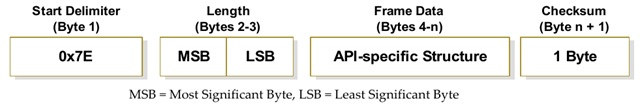
\includegraphics[width=.6\textwidth]{img/IMAGEN05.jpg}
\end{figure}
Donde cada parte corresponde a:

\begin{enumerate}
\item Byte 1: El encabezado que siempre tiene un valor de 0x7E,
  esto indica al módulo que está por comenzar la transmisión de un
  paquete.
\item Bytes 2, 3: Esta sección indica el tamaño del paquete, el
  tamaño se calcula contando los bits entre el byte menos
  significativo del tamaño y el byte de la suma de verificación
  (checksum).
\item Bytes 4-n: Esta sección contiene la estructura específica a
  la API, de los contenidos de esta parte del paquete dependerá la
  función de la API que se llame.
\item Byte n+1: La suma de verificación de todos los bytes
  contenidos en el paquete. Esto se utiliza para verificar la
  integridad de los datos recibidos, si la suma no coincide el
  paquete es descartado.
\end{enumerate}

El contenido del paquete de datos varía en base al comando que se quiera transmitir, por ejemplo si quisiéramos transmitir un dato a otro XBee utilizando una dirección de 16 bits deberíamos utilizar la siguiente estructura:
\begin{figure}[ht]
	\centering
	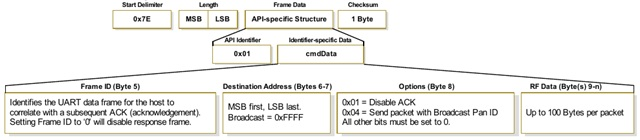
\includegraphics[width=.6\textwidth]{img/IMAGEN06.jpg}
\end{figure}

Configuración Frame ID a '0' desactivará trama de respuesta.
Donde la estructura tiene la siguiente forma:
\begin{enumerate}
	\item Byte 4:Identificador de la API, este código identifica el
      tipo de comando que queremos ejecutar, para este caso el código
      0x01 corresponde a Transmit Request: 16-Bit Address'' o solicitud de transmisión a una dirección de 16 bits.
	\item Byte 5:Corresponde a un número secuencial del paquete. Para cada envío se recibe un acuse de recibo'' (ACK) este número nos servirá luego para verificar que un paquete que enviamos fue recibido por el destinatario.
	\item Bytes 6, 7:Corresponden a la dirección del XBee destinatario, se coloca primero el byte más significativo y luego el menos significativo.
	\item Byte 8:Corresponde a las opciones de envío, si establecemos el bit 0x01 en 1 no se esperará un ACK, mientras que si habilitamos el bit 0x04 se enviará el mensaje con broadcast para todas las redes de área personal (PAN).
	\item Byte 9-n:Datos a enviar (máximo 100 bytes).
\end{enumerate}
\subsection{El modo API 1 y API 2}
Según la documentación del XBee existen dos modos API, la diferencia entre el modo 1 y el modo 2 es que en el Modo 2 las secuencias de bytes van ``escapadas''.

¿Qué significa esto? Resulta que el módulo XBee intentará leer el inicio de un paquete siempre encuentre el byte 0x7E, ¿pero qué pasa si este valor se está enviando en algún lugar dentro del paquete? Por ejemplo en el tamaño, o en la misma secuencia de datos.

Pues lo que ocurrirá será que el XBee va a descartar el paquete que estaba procesando y comenzará a procesar el nuevo de manera errónea. Para solventar este problema se incluyó el Modo API 2, en este modo antes de enviar un dato verificamos si el byte posee cualquiera de los siguientes valores:
\begin{itemize}
	\item 0x7E: Inicio del paquete.
	\item 0x7D: Carácter de escape.
	\item 0x11: Señalizador XON.
	\item 0x13: Señalizador XOFF.	
\end{itemize}
Para escapar la secuencia tenemos que enviar el carácter de escape más el dato que queremos enviar haciendo una operación XOR con el valor 0x20.
Por ejemplo, la secuencia del siguiente paquete:

0x7E 0x00 0x02 0x23 0x11 0xCB

Quedaría escapado de la siguiente manera:

0x7E 0x00 0x02 0x23 0x7D 0x31 0xCB

\subsection{Modo API}
Para habilitar el modo API debemos enviar la siguiente secuencia de comandos a nuestra XBee:
\subsubsection{Modo API 1:}
\begin{itemize}
	\item Enviamos ``+++'' y esperamos confirmaci\'on ``OK''.
	\item Enviamos ``ATAP1'' y esperamos confirmaci\'on ``OK''
	\item Enviamos ``ATCN'' y esperamos confirmaci\'on ``OK''
\end{itemize}
\subsubsection{Modo API 2:}
\begin{itemize}
	\item Enviamos ``+++'' y esperamos confirmaci\'on ``OK''.
	\item Enviamos ``ATAP2'' y esperamos confirmaci\'on ``OK''
	\item Enviamos ``ATCN'' y esperamos confirmaci\'on ``OK''
\end{itemize}
Una vez el XBee se encuentre en modo API, ignorará todos los datos que no muestren la secuencia correspondiente a una estructura de la API. Esto resulta muy útil ya que podemos imprimir sobre la misma línea Serie donde está conectado el XBee mensajes para ``depurar'' el funcionamiento y el XBee simplemente los ignorará.

Tomen en consideración que los datos recibidos del XBee también presentarán la estructura de la API así que leer los datos requerirá realizar el proceso detallado anteriormente pero a la inversa.

\subsubsection{Ejemplo de mensaje}
Si quisiéramos enviar el texto ``Hello World!'' en un broadcast, deberíamos enviar la siguiente secuencia de bytes al XBee:
\begin{lstlisting}[emph={0x7E:,0x00:,0x11:,0x01:,0xFF:,0xFF:,0x00:,
0x48:,0x65:,0x6C:,0x6C:,0x6F:,0x20:,0x57:,0x6F:,0x72:,0x6C:,0x64:,0x21:,
0xC3}, emphstyle={\color{blue}}, label=code:apiEjempl-id]
0x7E: Encabezado
0x00:
0x11: Tama\~no en Bytes del paquete (17)
0x01: Identificación del comando de la API (0x01 para enviar a dirección de 16 bits)
0x01: Identificación del paquete (cualquier número entre 0x01 y 0xFF)
0xFF: Byte más significativo dirección destino
0xFF: Byte menos significativo dirección destino
0x00: Opciones, ``0'' utiliza opciones por defecto.
0x48: 'H'
0x65: 'e'
0x6C: 'l'
0x6C: 'l'
0x6F: 'o'
0x20: ' '
0x57: 'W'
0x6F: 'o'
0x72: 'r'
0x6C: 'l'
0x64: 'd'
0x21: '!'
0xC3: Suma de verificación
\end{lstlisting}  
\subsubsection{La suma de verificación}
El último byte, la suma de verificación, se utiliza para garantizar que el paquete se haya transmitido de manera íntegra, lo calculamos restando a 0xFF la suma truncada a 8 bits de todos los bytes entre el tamaño del paquete y el checksum, para el ejemplo anterior la fórmula del checksum sería:


0xFF- 0xFF \&(0x01+ 0xFF+ 0xFF+ 0x00+0x48+
0x65+ 0x6C+ 0x6C+0x6F + 0x20 +
0x57+ 0x6F+0x72 +0x6C + 0x64+0x21) = 0xC3


Utilizando el software XCTU y comandos AT en modo API, configurar dos entradas como canales de conversión AD. Utilizar el comando ATIS para leer las entradas. Describir el significado de la información devuelta por el modulo luego del envió de este comando.
\begin{figure}[ht]
	\centering
	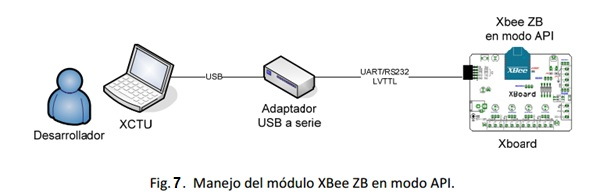
\includegraphics[width=.6\textwidth]{img/IMAGEN07.jpg}
\end{figure}
Al igual que en el modo AT, las configuraciones de los puertos son similares, con la salvedad de que debemos enviar el comando AT dentro de una trama API especialmente diseñada para enviar comandos AT.

El software XCTU cuenta con, entre otras herramientas, con un frame generator y un frame interpreter especialmente diseñados para poder crear e interpretar tramas API.

Estas dos utilidades se muestran a continuación

\begin{figure}[ht]
	\centering
	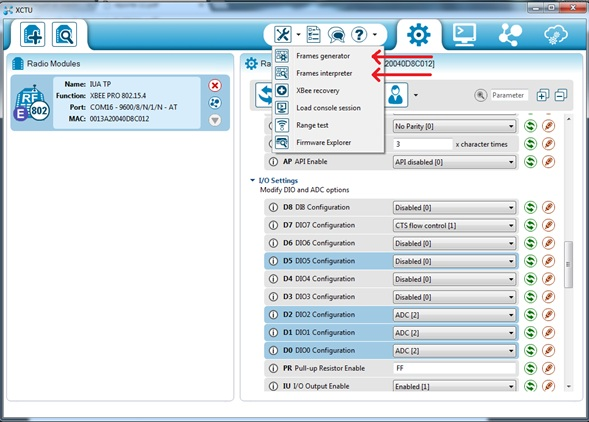
\includegraphics[width=.6\textwidth]{img/IMAGEN08.jpg}
	\caption{Ubicaci\'on del frame generador e interprete dentro de XCTU}
\end{figure}
A continuación veremos cómo utilizar el frame generator:
\begin{figure}[ht]
	\centering
	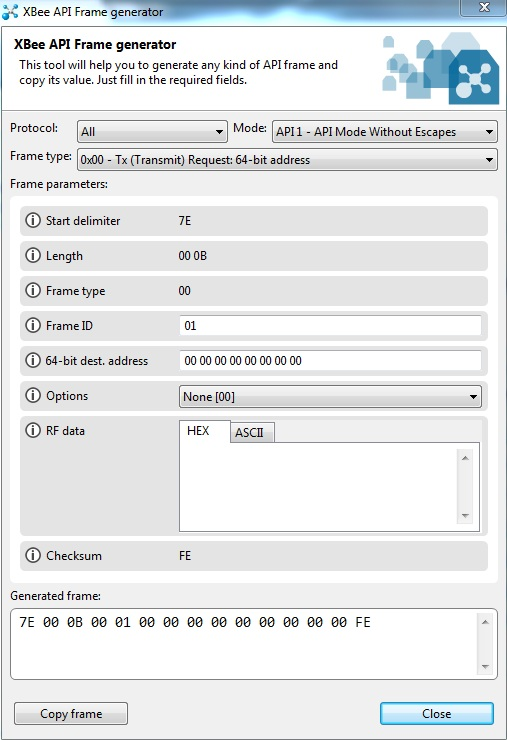
\includegraphics[width=.6\textwidth]{img/IMAGEN09.jpg}
	\caption{``Frame generator'' de XCTU}
\end{figure}
Dentro del marco de generaci\'on, podemos encontrar varias opciones:
\begin{itemize}
	\item Tipo de protocolo: 802.15. Wi-Fi, XTend(digimesh), Xted(Legacy), ZigBee, DigiMesh, Point to multipoint, ZNet 2.5,Smart Energy, XLR.
	\item Modo: API1-Modo API no escapado, API2-Modo API escapado.
	\item Tipo de frame: Dependiendo de lo que vayamos a transmitir, 2 bytes con opciones desde 0x00h a 0xFFh.
	\end{itemize}
	Además, tenemos una lista de todos los bytes que componen la trama API, explicando cada uno de ellos, como la sig.
\begin{figure}[ht]
		\centering
		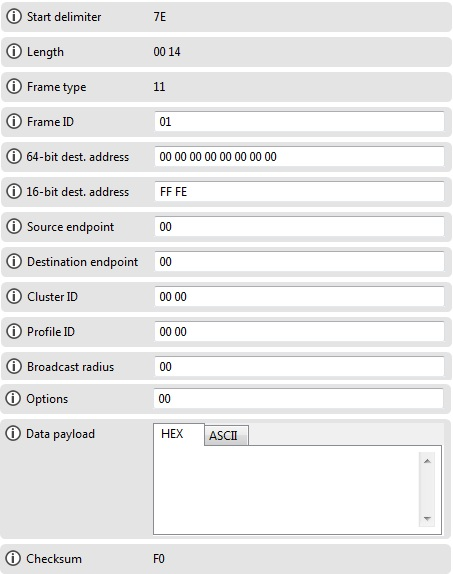
\includegraphics[width=.6\textwidth]{img/IMAGEN10.jpg}
		\caption{Trama API dentro del marco generador.}
\end{figure}
Al colocar todos los parámetros pertinentes para crear la trama API, así como el payload que vamos a enviar, ya sea este un comando AT o caracteres ASCII, podremos ver el frame generado en la parte inferior del frame generator y podremos copiarlo al portapapeles con el botón “copy frame”
\begin{figure}[ht]
	\centering
	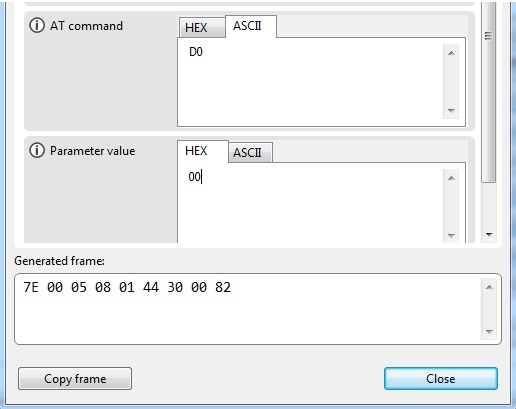
\includegraphics[width=.6\textwidth]{img/IMAGEN11.jpg}
	\caption{Frame generado con el Frame Generator.}
\end{figure}
Este frame que copiamos, es el que vamos a utilizar en la consola para poder enviar informacion.
\begin{figure}[ht]
	\centering
	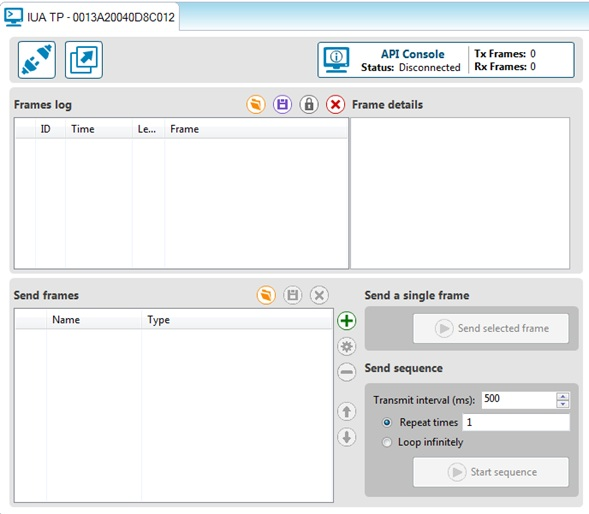
\includegraphics[width=.6\textwidth]{img/IMAGEN12.jpg}
	\caption{Consola de comandos API.}
\end{figure}
Acto seguido presionamos el botón “+” verde y veremos la siguiente pantalla.
\begin{figure}[h]
	\centering
	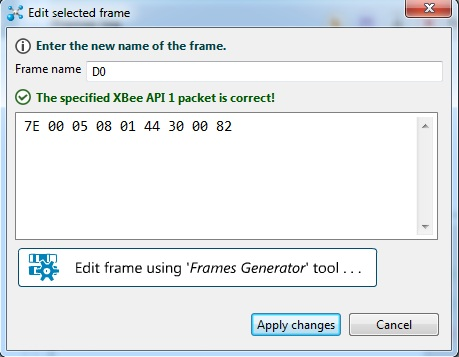
\includegraphics[width=.6\textwidth]{img/IMAGEN13.jpg}
	\caption{Agregando una nueva trama API a la lista de comandos}
\end{figure}
Dentro de esta pantalla podemos ver que tenemos acceso al Frame generator, con lo cual como antes vimos, crearemos nuestra trama API, en este caso creamos la trama API de comandos AT, para enviar el comando “ATD00”, que nos sirve para deshabilitar el puerto D0 por ejemplo.

Enviamos el frame con el botón verde “Send selected frame”.

\begin{figure}[h]
	\centering
	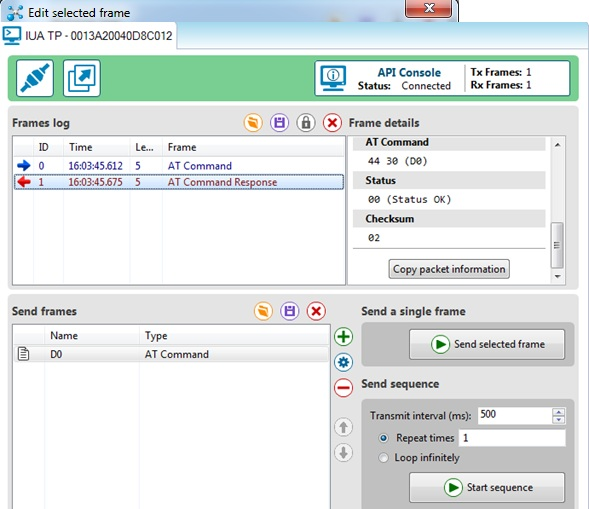
\includegraphics[width=.6\textwidth]{img/IMAGEN14.jpg}
	\caption{Envió del frame generado para deshabilitar el puerto D0}
\end{figure}

En la parte derecha de la consola podremos ver los detalles de cada frame como “AT Command” o “AT Command response” donde sabremos si el comando tuvo efecto sobre el puerto en cuestión.

Podemos copiar esa respuesta en el portapapeles con el botón “copy packet information” y lo vemos como sigue:
\begin{lstlisting}[emph={AT, Command, Response, (API 1),Start, delimiter:,Length:,Frame, type:,Frame, ID:,AT, Command:,Status:,Checksum: }, emphstyle={\color{green}}, label=code:apiEjempl-id]
AT Command Response (API 1)
7E 00 05 88 01 44 30 00 02
Start delimiter:
7E
Length:
00 05 (5)
Frame type:
88 (ATCommandResponse)
Frame ID:
01 (1)
AT Command:
44 30 (D0)
Status:
00 (Status OK)
Checksum:
02
\end{lstlisting}  
En el ejemplo anterior vimos como desactivar una entrada del GPIO, ahora como se solicitó en el práctico mostraremos la secuencia para configurar dos entradas como canales de conversión AD. Y luego leeremos la información con el comando ATIS.
Vamos a generar una lista de tramas para enviar desde la consola API del XCTU y de ese modo poder configurar los puertos como se pidió.
Los comandos que vamos a enviar en tramas API serán los siguientes:
\begin{lstlisting}[emph={ATD02:, Trama API:,ATD12:,ATWR:,ATAC:,}, emphstyle={\color{green}}, label=code:apiEjempl-id]
ATD02: Configuramos la entrada D0 como puerto analógico.
Trama API: 7E 00 05 08 01 44 30 02 80
ATD12: Configuramos la entrada D1 como puerto analógico.
Trama API: 7E 00 05 08 01 44 31 02 7F
ATWR: Guardamos los cambios en la memoria.
Trama API: 7E 00 04 08 01 57 52 4D
ATAC: Aplica los cambios al módulo.
Trama API: 7E 00 04 08 01 41 43 72
\end{lstlisting}  
\begin{figure}[h]
	\centering
	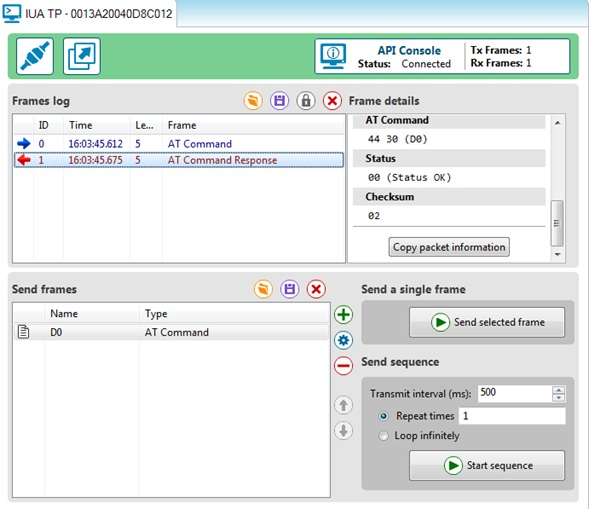
\includegraphics[width=.6\textwidth]{img/IMAGEN15.jpg}
	\caption{Entradas del GPIO antes de aplicar las tramas API.}
\end{figure}
En la esquina inferior derecha veremos un botón verde ``Start
sequence'', este botón envía los 4 frames directamente y guarda los
cambios ocupando los comandos anteriormente mencionados. 
\begin{figure}[h]
	\centering
	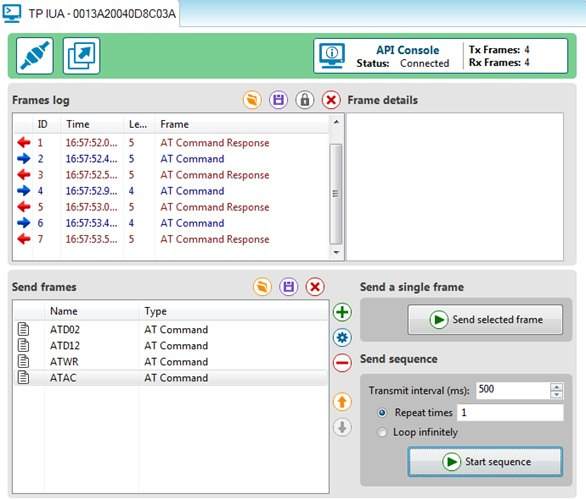
\includegraphics[width=.6\textwidth]{img/IMAGEN16.jpg}
	\caption{Envió de la secuencia de tramas para configurar el GPIO.}
\end{figure}
\begin{figure}[h]
	\centering
	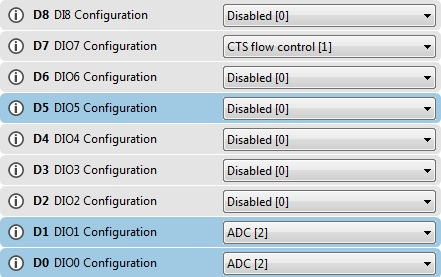
\includegraphics[width=.6\textwidth]{img/IMAGEN17.jpg}
	\caption{Estado del GPIO luego de la configuración.}
\end{figure}

Ahora vamos a configurar dos entradas digitales.
Los comandos que vamos a enviar en tramas API serán los siguientes:
\begin{lstlisting}[emph={ATD03:,Trama API:,ATD13:,ATWR:,ATAC:}, emphstyle={\color{green}}, label=code:apiEjempl-id]
ATD03: Configuramos la entrada D0 como puerto analógico.
Trama API: 7E 00 05 08 01 44 30 03 7F
ATD13: Configuramos la entrada D1 como puerto analógico.
Trama API: 7E 00 05 08 01 44 31 03 7E
ATWR: Guardamos los cambios en la memoria.
Trama API: 7E 00 04 08 01 57 52 4D
ATAC: Aplica los cambios al módulo.
Trama API: 7E 00 04 08 01 41 43 72
\end{lstlisting} 

\begin{figure}[h]
	\centering
	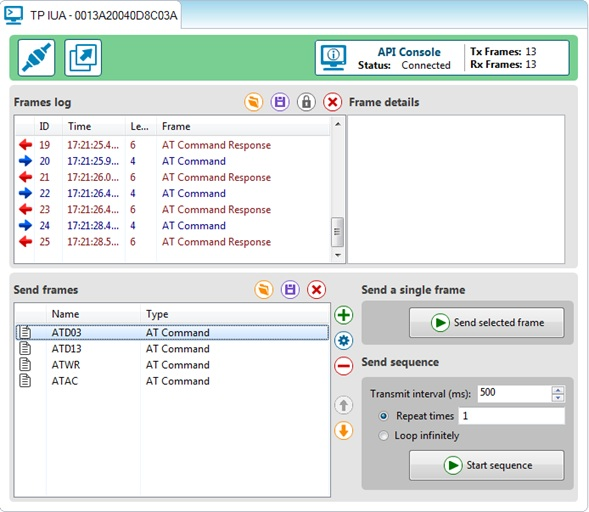
\includegraphics[width=.6\textwidth]{img/IMAGEN18.jpg}
	\caption{Envió de la secuencia de tramas para configurar el GPIO.}
\end{figure}
\begin{figure}[h]
	\centering
	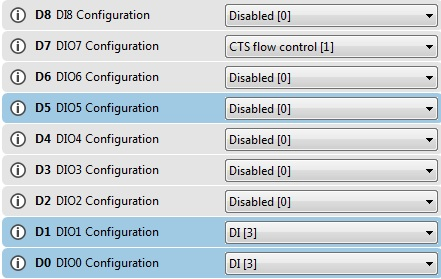
\includegraphics[width=.6\textwidth]{img/IMAGEN19.jpg}
	\caption{Estado del GPIO luego de la configuración.}
\end{figure}
Ahora vamos a configurar dos salidas digitales.
Los comandos que vamos a enviar en tramas API serán los siguientes:
\begin{lstlisting}[emph={ATD04: ,Trama API:,ATD14:,ATWR:,ATAC:}, emphstyle={\color{green}}, label=code:apiEjempl-id]
ATD04: Configuramos la entrada D0 como puerto analógico.
Trama API: 7E 00 05 08 01 44 30 04 7E
ATD14: Configuramos la entrada D1 como puerto analógico.
Trama API: 7E 00 05 08 01 44 31 04 7D
ATWR: Guardamos los cambios en la memoria.
Trama API: 7E 00 04 08 01 57 52 4D
ATAC: Aplica los cambios al módulo.
Trama API: 7E 00 04 08 01 41 43 72
\end{lstlisting} 
\begin{figure}[h]
	\centering
	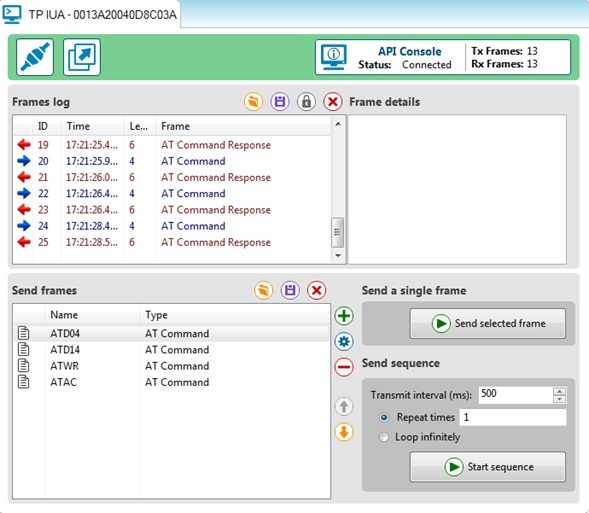
\includegraphics[width=.6\textwidth]{img/IMAGEN20.jpg}
	\caption{Envió de la secuencia de tramas para configurar el GPIO.}
\end{figure}
\begin{figure}[h]
	\centering
	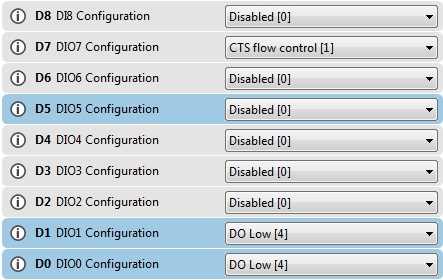
\includegraphics[width=.6\textwidth]{img/IMAGEN21.jpg}
	\caption{Estado del GPIO luego de la configuración.}
\end{figure}
Empleo del comando ATIS.

Para probar este comando vamos a configurar las dos primeras entradas analógicas y las dos siguientes digitales.
Los comandos que vamos a enviar en tramas API serán los siguientes:
\begin{lstlisting}[emph={ATD02: ,Trama API:,ATD12:,ATD23:,ATD33:,ATWR:,ATAC:,ATIS:}, emphstyle={\color{green}}, label=code:apiEjempl-id]
ATD02: Configuramos la entrada D0 como puerto analógico.
Trama API: 7E 00 05 08 01 44 30 32 50
ATD12: Configuramos la entrada D1 como puerto analógico.
Trama API: 7E 00 05 08 01 44 31 32 4F
ATD23: Configuramos la entrada D1 como puerto analógico.
Trama API: 7E 00 05 08 01 44 32 33 4D
ATD33: Configuramos la entrada D1 como puerto analógico.
Trama API: 7E 00 05 08 01 44 33 33 4C
ATWR: Guardamos los cambios en la memoria.
Trama API: 7E 00 04 08 01 57 52 4D
ATAC: Aplica los cambios al módulo.
Trama API: 7E 00 04 08 01 41 43 72
ATIS: se utiliza para forzar una lectura de todas las líneas ADC/DIO habilitadas
Trama API: 7E 00 04 08 12 49 53 49
\end{lstlisting} 
\begin{figure}[h]
	\centering
	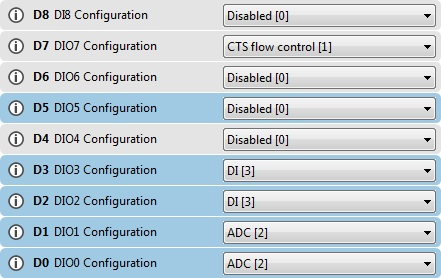
\includegraphics[width=.6\textwidth]{img/IMAGEN22.jpg}
	\caption{Estado del GPIO luego de la configuración.}
\end{figure}
Luego del envió de la secuencia de tramas para configurar el GPIO enviamos la trama con el comando ATIS y la misma nos devuelve lo siguiente:
\begin{lstlisting}[emph={RX,(,Receive,),Packet,16,-,bit,Address,IO,(API, 1),Start,delimiter:,Length:,Frame, type:,16-bit, source, address:, RSSI:,Options:,Number, of, samples:,Digital, channel, mask:,Analog ,channel mask: ,DIO2/AD2, digital, value: ,DIO3/AD3, DIO0/AD0, analog}, emphstyle={\color{black}}, label=code:apiEjempl-id]
RX (Receive) Packet 16-bit Address IO (API 1)
7E 00 0E 83 00 00 00 00 01 06 0C 00 0C 03 FF 03 FF 59
Start delimiter:        7E
Length:                 00 0E (14)
Frame type:  83 (RX(Receive)Packet16-bitAddressIO)
16-bit source address:  00 00
RSSI:                   00
Options:                00
Number of samples:      01
Digital channel mask:   00 0C
Analog channel mask:    06 00
DIO2/AD2 digital value: High
DIO3/AD3 digital value: High
DIO0/AD0 analog value:  03 FF (1023)
DIO1/AD1 analog value:  03 FF (1023)
Checksum:               59
\end{lstlisting} 
El último Frame enviado, nos devuelve una respuesta que es el estado
de las líneas activas, en este caso el estado de las dos entradas
analógicas en 03FF (1023) y las dos entradas digitales en High.

%=============== SEBA ==========


\section{Enlaces entre módulos XBee}
\label{sec:enlace}

Ya se mostraron en las secciones anteriores las diferentes formas de
manipular los módulos XBee. En esta sección se desarrollarán pruebas
de enlace de los módulos. Las características de radio frecuencia no
son objeto de estudio, se busca evaluar las virtudes en la red que
implementa el estándar 802.15.4. Se utilizará la topología más
sencilla del alcance de las redes Zigbee. Se implementará un
\emph{Coordinador} y los demás serán configurados como
\emph{Dispositivos finales}. En la Figura \ref{fig:xbee-red} se presenta
una red de módulos XBee en las que se puede ver las diferentes
roles que pueden asumir estos dispositivos. A parte de los dos modos
anteriormente nombrados se puede configurar en modo \emph{router} que
permite extender la red. 

\begin{figure}[h]
  \centering
  \includegraphics[width=.8\textwidth]{img/xbee-topo}
  \caption{Red de módulos XBee con sus diferentes configuraciones.}
  \label{fig:xbee-red}
\end{figure}

\subsection{Asignación de Identificador y Función de los módulos}

Antes de comenzar con la configuración de la red, se definirá a uno de
los módulos como coordinador y los demás como dispositivos
finales. Además proporcionaremos un nombre para identificarlos a cada
uno ellos. En la línea \textbf{4} del código
\ref{code:coordinador-id}  se habilita el modo coordinador y luego se
asigna el nombre \texttt{COORDINADOR} al módulo (línea \textbf{8}).
 Como en los casos anteriores, seimpre se debe aplicar los cambios (\texttt{ATAC}) y
finalmente escribir en la memoria no-volatil (\texttt{ATWR}).
\begin{lstlisting}[emph={+++,ATCE,ATCE1,ATWR,ATAC,ATNI,ATCOORDINADOR},
    emphstyle={\color{blue}}, caption={Obtención del \textsl{seral
number}.}, label=code:coordinador-id]
+++OK
ATCE
0
ATCE1
OK
ATCE
1
ATNICOORDINADOR
OK
ATNI
COORDINADOR
ATAC
OK
ATWR
OK
\end{lstlisting}  

\subsection[Configuración PAN]{Configuración de la red de área personal}

Las redes ZigBee se las llaman PANs (\textsl{Personal Area
  Networks}). Cada red es definida con un único identificador PAN, por
lo que todos los dispositivos que quieran pertenecer a la red deben
tener el mismo \texttt{ID PAN}. 

ZigBee soporta tanto PAN ID de 16 a 64 bits. Ambos PAN IDs son
utilizados como único identificador de la red. Los dispositivos que
quieran integrar la misma red deberán compartir el mismo PAN IDs. 

En el código \ref{code:pan-id} se asigna el PAN ID \texttt{260816} al
módulo coodinador y será el mismo que utilizarán los demás
dispositivos para conectarse a la red ZigBee. En la línea \textbf{2}
se solicita el actual PAN ID y el módulo responde \texttt{0}. Luego se
aplica el identificador \texttt{260816}, se utilizan solo 24 de los
los 64 bits disponibles. 

\begin{lstlisting}[emph={+++,ATWR,ATAC,ATID,ATID260816},
    emphstyle={\color{blue}}, caption={Obtención del \textsl{serial
number}.}, label=code:pan-id]
+++OK
ATID
0
ATID260816
OK
ATID
260816
ATAC
OK
ATWR
OK
\end{lstlisting}  

\subsection[Número de serie]{Número de serie (identificador)  los módulos}
\label{sec:id}

Cada módulo XBee tiene una número de serie de 64 bits
(\textsl{extended address}) grabado en el \textsl{hardware} por el
fabricante\footnote{Recuerde que también los XBee tienen un
  direccionamiento de 16 bits. Para mayor información ver la
  bibliografía.}. Mediante los comandos AT se puede obtener
esta dirección en dos partes. Los comandos \texttt{ATSH} y
\texttt{ATSL} devuelven la parte alta y baja respectivamente. Estos
valores se utilizan para la configuración de la red Zigbee (junto a
los valores de  los demás módulos). En
el código \ref{code:get-id}  se muestra cómo obtener el número de serie
del dispositivo al que se encuentra conectado el terminal
serial. 
\begin{lstlisting}[emph={+++,ATSH,ATSL},
    emphstyle={\color{blue}}, caption={Obtener el \textsl{serial
        number} del módulo XBee},
 label=code:get-id]
+++OK
ATSH
13A200
ATSL
41257816
\end{lstlisting}

\subsection[Direeccionamiento]{Configuración de direccionamiento de los dispositivos en
  una red ZigBee}

En la sección anterior se mostró como obtener las identificaciones de
cada módulo. Esta información se utiliza para mapear la red a
implementar. Se recuerda que la topología utilizada en estos
prácticos, se tendrá un coordinador y varios dispositivos finales que
proporcionarán información al primero. En este caso el coordinador
configura su dirección de destino al único (por el momento)
dispositivo conectado, código \ref{code:coord-dest}. Se cargan la
parte alta (\texttt{ATDH13A200}) y la baja (\texttt{ATDL4125768A}) con
los valores propios del dispositivo final al que se conectará el
coordinador. En forma recíproca se debe cargar el identificador del
coordinador como dirección de destino del único dispositivo final
conectado a la red. Esto último se muestra en el código
\ref{code:end-dest}. Para mejor entendimiento de los códigos de
configuración se solicita antes a los módulos responder el nombre que
identifica a los módulos y sus respectivos números de serie. Al final
se guardan todos los cambios realizados.

\noindent\begin{minipage}{.45\textwidth}
\begin{lstlisting}[emph={+++,ATWR,ATAC,ATNI,ATSH,ATSL,ATDH13A200,ATDL4125768A},
emphstyle={\color{blue}}, caption={Destino del coordinador.},label=code:coord-dest]
+++OK
ATNI
COORDINADOR
ATSH
13A200
ATSL
41257816
ATDH13A200
OK
ATDL4125768A
OK
ATAC
OK
ATWR
OK
\end{lstlisting}  
\end{minipage}\hfill
\begin{minipage}{.45\textwidth}
\begin{lstlisting}[emph={+++,ATWR,ATAC,ATSH,ATNI,ATSL,ATDH13A200,ATDL41257816},
emphstyle={\color{blue}}, caption={Destino del coordinador.},label=code:end-dest]
+++OK
ATNI
DISPOSITIVO1
ATSH
13A200
ATSL
4125768A
ATDH13A200
OK
ATDL41257816
OK
ATAC
OK
ATWR
OK
\end{lstlisting}  
\end{minipage}

\subsection[Enlace a través de Xbee]{Comunicación entre computadoras mediante módulos XBee}

Con los módulos configurados anteriormente para establecer una
comunicación punto a punto, se probará el enlace entre los módulos
comunicando ambos módulos entre sí mediante un terminal de
computadora. Es decir, se utilizarán dos computadoras conectando sus
respectivos puertos seriales (RS232) a cada módulo XBee ya
configurados. A continuación se presentan las capturas de pantalla de
dos terminales. En la Figura \ref{fig:term-coord} se muestran la
consola de XCTU del coordinador. Mientras que en la Figura
\ref{fig:term-end} se ven los mensajes recibidos desde el terminal del
dispositivo conectado a la red ZigBee (\texttt{DISPOSITIVO 1}).

\begin{figure}[h]
  \centering
  \begin{subfigure}{0.8\textwidth}
    \centering
    \includegraphics[width=\textwidth]{img/terminal-coord}
    \caption{Consola con el módulo coordinador.}
    \label{fig:term-coord}
  \end{subfigure}
  % --
  \begin{subfigure}{0.8\textwidth}
    \centering
    \includegraphics[width=\textwidth]{img/terminal-dispo}
    \caption{Consola con el módulo conectado a la red.}
    \label{fig:term-end}
  \end{subfigure}
  % --
  \caption{Captura de pantalla de las consolas utilizando XCTU.}
  \label{fig:terminales}
\end{figure}

\section{Control remoto de los módulos XBee}
\label{sec:remoto}

En la Sección \ref{sec:API} se realizaron pruebas de los módulos en modo
API. Este modo introduce complejidad pues debe generarse una trama
específica pero de esta forma se logra mayores prestaciones por parte
de los módulos. 

En el siguiente ejemplo se describirá el mecanismo por el cual se
configura el comportamiento de un módulo XBee en forma remota desde
otro. Los módulos debe estar ya configurados como se describió
anteriormente. Se utilizará el \emph{Generador de Frames}, aplicativo
del software XCTU. 

En la Figura \ref{fig:remotos-dio5} se capturan la generación de
comandos enviados desde el módulo coordinador a uno de sus
dispositivos conectados. Primero se releva el estado del módulo, esto
con el comando \texttt{ATIS} (Fig. \ref{fig:remoto-atis}). Aquí se
ingresa la dirección destino del módulo al que se le enviará el
comando. Luego de chequear el estado de los puertos se enviará un
comando para asignar un estado bajo al puerto \texttt{DIO5}
(Fig. \ref{fig:remoto-atd54}). De la misma forma, se envía un comando
al puerto 5 con el cambio de estado \texttt{ATD55}
(Fig. \ref{fig:remoto-atd55}).

\begin{figure}[h]
  \centering
  \begin{subfigure}{0.3\textwidth}
    \centering
    \includegraphics[width=\textwidth]{img/remoto-atis}
    \caption{Comando \texttt{ATIS}.}
    \label{fig:remoto-atis}
  \end{subfigure}
  % -- 
  \hfill
  \begin{subfigure}{0.3\textwidth}
    \centering
    \includegraphics[width=.86\textwidth]{img/remoto-td54}
    \caption{Comando \texttt{ATD54}.}
    \label{fig:remoto-atd54}
  \end{subfigure}
  % --
  \hfill
  \begin{subfigure}{0.3\textwidth}
    \centering
    \includegraphics[width=\textwidth]{img/remoto-atd55}
    \caption{Comando \texttt{ATD55}.}
    \label{fig:remoto-atd55}
  \end{subfigure}
  % --
  \caption{Comandos remotos desde un módulo a otro.}
  \label{fig:remotos-dio5}
\end{figure}

Los comandos AT se encuentran concatenados con los caracteres propios
de la trama definida por el API. Por lo tanto, la clave es las
funcionalidades y prestaciones del \textsl{interface}. Se podría enviar los
mismos comandos AT de la Sección \ref{sec:AT} sin problemas. Pues la
trama API identifica qué tipo de información se está enviando.


\section{Librería \texttt{xbee-arduino}}
\label{sec:lib-xbe-ano}

Esta librería permite la comunicación con los módulos XBee en modo
API. Tiene soporte tanto para los dispositivos \emph{Series 1}
(802.15.4) y \emph{Series 2} (ZB Pro/ZNet). De esta forma la librería
da soporte para enlaces TX/RX, comandos AT locales y remotos, modos
I/O \textsl{samples} y \textsl{Modem Status}\cite{XbeeArduinoGit}.

La plataforma arduino que se utilizará será la \emph{Intel
  Galileo}, Figura \ref{fig:galileo}. Esta plataforma está basada en el microcontrolador
\emph{Intel\textsuperscript{\textregistered{}} Quark SoC X1000 Application
  Processor}. Las características de esta plataforma se detallan en la
hoja de datos disponibles en la bibliografía
citada\cite{GalileoDS}. Sí bien esta plataforma es una
SBC\footnote{Siglas de \textsl{Single-Board
    Computer}(\burl{https://en.wikipedia.org/wiki/Single-board_computer}).}
dispone de un proceso en el sistema operativo tal que permite utilizar
el IDE Arduino. Para el usuario la programación es transparente e
incluso la placa Galileo permite conectar los \textsl{shields} de
Arduino. Utilizaremos estos conectores para comunicar nuestros módulos
XBee con la Galileo.
\begin{figure}[h]
  \centering
  \begin{subfigure}{0.55\textwidth}
    \centering
    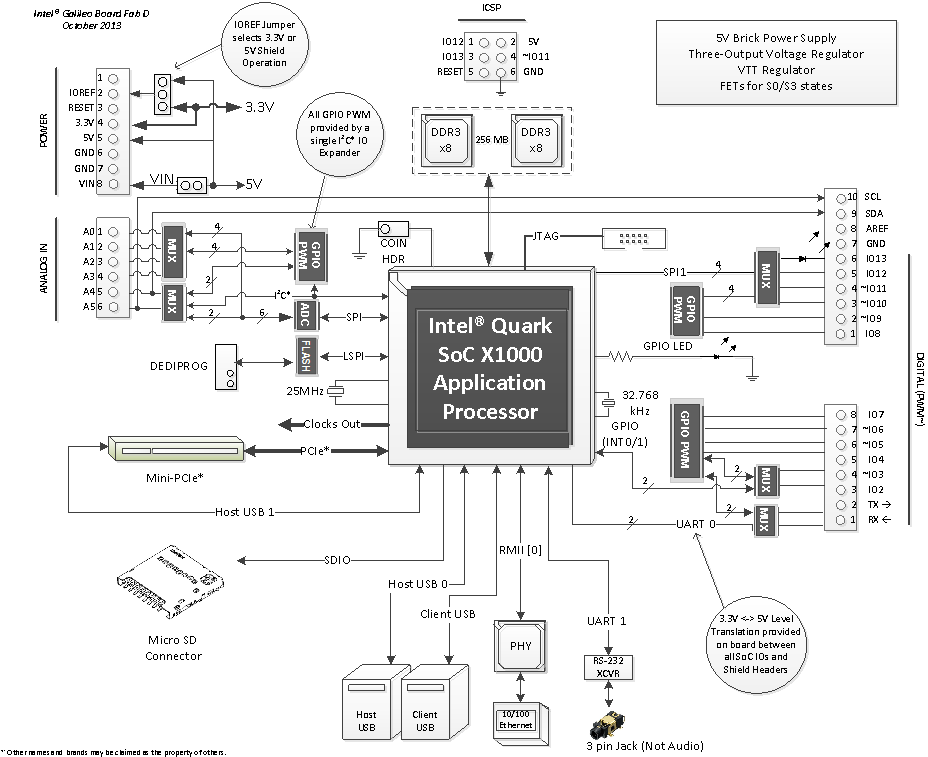
\includegraphics[width=\textwidth]{img/galileo.png}
    \caption{Diagrama en bloque.}
    \label{fig:sch-galileo}
  \end{subfigure}
  % -- 
  \hfill
  \begin{subfigure}{0.4\textwidth}
    \centering
    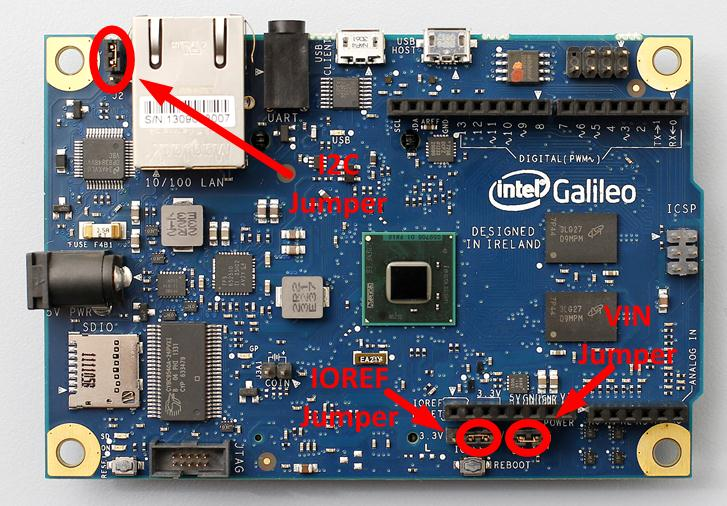
\includegraphics[width=\textwidth]{img/galileo-front}
    \caption{Pines de configuración.}
    \label{fig:galileo-config}
  \end{subfigure}

  \caption{Plataforma Intel\textsuperscript{\textregistered{}} Galileo.}
  \label{fig:galileo}
\end{figure}

Una vez instalada la librería desde los repositorios de Arduino se
procede a iniciar la comunicación entre la plataforma Galileo y el
módulo XBee. 

\subsection{Comandos AT}

La primera prueba será enviar comandos AT desde la Galileo hacía el
módulo XBee conectado en los conectores disponibles. En el código
\ref{code:at-cmd} se muestra la estructura básica de cómo se debe
utilizar la librería \texttt{xbee-arduino}. 
\begin{lstlisting}[basicstyle=\ttfamily\small, language= C++,
  caption={Ejemplo \texttt{AtCommand}},label=code:at-cmd, frame=single]
#include <XBee.h>
XBee xbee = XBee();
// serial high
uint8_t shCmd[] = {'S','H'};
// serial low
uint8_t slCmd[] = {'S','L'};

AtCommandRequest atRequest = AtCommandRequest(shCmd);
AtCommandResponse atResponse = AtCommandResponse();

void setup() { 
  Serial1.begin(9600);
  xbee.begin(Serial1);
  // start soft serial
  Serial.begin(9600);

  // Startup delay to wait for XBee radio to initialize.
  // you may need to increase this value if you are not getting a response
  delay(5000);
}

void loop() {

  // get SH
  sendAtCommand();
    
  // set command to SL
  atRequest.setCommand(slCmd);  
  sendAtCommand();
   
  // we're done.  Hit the Arduino reset button to start the sketch over
  while (1) {};
}
\end{lstlisting}  

En este documento no se explicará el paradigma de programación de
Arduino, tampoco se entrará en detalle de los códigos utilizados. De
todas formas se explicarán las códigos que hacen el uso de la librería
\texttt{xbee-arduino}. En las líneas \textbf{8-9} se crean los objetos
correspondientes a la recepción y respuesta de un comando AT. Se
habilitarán dos puertos de la Galileo. El primero (línea \textbf{12})
corresponde al puerto mapeado al conector \textsl{shield}
arduino. Este será asignado para que la librería \texttt{xbee-arduino}
la utilice en su comunicación con el módulo. El puerto serie que está
vinculado al cable USB conectado con la placa galileo será utilizado
como \emph{Monitor Serial} del IDE Arduino (línea \textbf{15}). Ya en
el bucle \texttt{loop()} se envían los comandos y se interpreta
consecutivamente la respuesta desde el módulo.  En la Figura
\ref{fig:at-cmd-consola} se puede ver el intercambio de mensajes entre
la Galileo y el módulo XBee.
\begin{figure}[h]
  \centering
  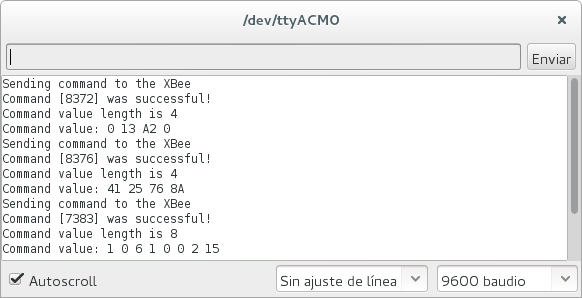
\includegraphics[width=.5\textwidth]{img/arduno-at-cmd.png}
  \caption{Monitor serial del IDE Arduino del ejemplo \texttt{AtCommand}.}
  \label{fig:at-cmd-consola}
\end{figure}

\subsection[Ejemplo \texttt{Series2\_Tx/\_Rx}]{Comunicación entre dos
  plataformas Galileo utilizando XBee.}

Se plantea la posibilidad de utilizar dos plataformas Galileo e
interactuar entre sí utilizando los módulos XBee como medio de
comunicación. Se adaptará los ejemplos provistos por la
librería. Primero se adaptará el ejemplo \texttt{Series2\_Tx}. 

\subsubsection{Transmisión de trama}

En el código \ref{code:SeriesTx} se tiene las principales líneas que
implementa la librería. El arreglo \texttt{payload[]} almacena los
datos a ser enviados. Por la inicialización del arreglo, se enviarán
solo dos bytes (línea \textbf{6}). Luego se crean los objetivos
necesarios para direccionar el mensaje, realizar el envío y chequear
el estado de la transacción (líneas \textbf{9-11}). Se enviarán los
valores devueltos por la función \texttt{millis()} y
\texttt{micros()} (líneas \textbf{25-26}). El proceso cíclico comienza
cargando los datos a ser enviado (línea \textbf{28}). Luego del envío
se espera el paquete de respuesta. Esta respuesta proporciona el
estado en que ha sido recibido el mensaje (línea \textbf{40}). Esto se
repite cada 1 segundo (línea \textbf{55}). 

\begin{lstlisting}[basicstyle=\ttfamily\small, language= C++,
  caption={Ejemplo \texttt{Series2\_Tx}},label=code:SeriesTx,
  frame=single]
#include <XBee.h>

// create the XBee object
XBee xbee = XBee();

uint8_t payload[] = { 0, 0 };

// SH + SL Address of receiving XBee
XBeeAddress64 addr64 = XBeeAddress64(0x0013a200,0x41257816);
ZBTxRequest zbTx = ZBTxRequest(addr64, payload, sizeof(payload));
ZBTxStatusResponse txStatus = ZBTxStatusResponse();

//...

void setup() {
  pinMode(statusLed, OUTPUT);
  pinMode(errorLed, OUTPUT);

  Serial1.begin(9600);
  xbee.setSerial(Serial1);
}

void loop() {   
  // break down 10-bit reading into two bytes and place in payload
  payload[0] = millis() & 0xff;
  payload[1] = micros() & 0xff;

  xbee.send(zbTx);

  // after sending a tx request, we expect a status response
  // wait up to half second for the status response
  if (xbee.readPacket(500)) {
    // got a response!

    // should be a znet tx status            	
    if (xbee.getResponse().getApiId() == ZB_TX_STATUS_RESPONSE) {
      xbee.getResponse().getZBTxStatusResponse(txStatus);

      // get the delivery status, the fifth byte
      if (txStatus.getDeliveryStatus() == SUCCESS) {
        // success.  time to celebrate
        flashLed(statusLed, 5, 50);
      } else {
        // the remote XBee did not receive our packet. is it powered on?
        flashLed(errorLed, 3, 500);
      }
    }
  } else if (xbee.getResponse().isError()) {
    //nss.print("Error reading packet.  Error code: ");  
    //nss.println(xbee.getResponse().getErrorCode());
  } else {
    // local XBee did not provide a timely TX Status Response -- should not happen
    flashLed(errorLed, 2, 50);
  }
  delay(1000);
}
\end{lstlisting}  

\subsubsection{Recepción  de trama}

Desde otra plataforma Galileo se adapta el ejemplo
\texttt{Series2\_Rx} de la librería \texttt{xbee-arduino}. El código
\ref{code:SeriesRx} muestra lo básico. Las primeras líneas mantienen
la estructura del ejemplo anterior. Los objetos que se crean hacen a
la respuesta ante algún pedido desde otro módulo. Se utilizará el
monitor del IDE Arduino para presentar los datos recibidos (línea
\textbf{17}). El bucle se encuentra a la espera de un paquete (línea
\textbf{26}). Una vez que el paquete llega (línea \textbf{28}) se
procede a identificar los diferentes campos de bytes de la trama. Se
utilizan indicadores leds que proporcionan los estados en que llega la
trama. Luego se presentan los bytes enviados desde el otro módulo. Las
líneas \textbf{46} y \textbf{48} imprimen en la consola del IDE
arduino. 

\begin{lstlisting}[basicstyle=\ttfamily\small, language= C++,
  caption={Ejemplo \texttt{Series2\_Rx}},label=code:SeriesRx,
  frame=single]
#include <XBee.h>

XBee xbee = XBee();
XBeeResponse response = XBeeResponse();
// create reusable response objects for responses we expect to handle 
ZBRxResponse rx = ZBRxResponse();
ModemStatusResponse msr = ModemStatusResponse();

int statusLed = 13;
int errorLed = 12;

void setup() {
  pinMode(statusLed, OUTPUT);
  pinMode(errorLed, OUTPUT);
  
  // start serial
  Serial.begin(9600);
  Serial1.begin(9600);
  xbee.begin(Serial1);

}

// continuously reads packets, looking for ZB Receive or Modem Status
void loop() {
    
    xbee.readPacket();
    
    if (xbee.getResponse().isAvailable()) {
      // got something
      
      if (xbee.getResponse().getApiId() == ZB_RX_RESPONSE) {
        // got a zb rx packet
        
        // now fill our zb rx class
        xbee.getResponse().getZBRxResponse(rx);
            
        if (rx.getOption() == ZB_PACKET_ACKNOWLEDGED) {
            // the sender got an ACK
            // ...
        } else {
            // we got it (obviously) but sender didn't get an ACK
            // ...
        }
        // set dataLed PWM to value of the first byte in the data
        Serial.print("Mensaje recibido (LOW): ");
        Serial.println(rx.getData(0));
        Serial.print("Mensaje recibido (HIGH): ");
        Serial.println(rx.getData(1));
      } else if (xbee.getResponse().getApiId() == MODEM_STATUS_RESPONSE) {
        // ...
    } else if (xbee.getResponse().isError()) {
      Serial.print("Error reading packet.  Error code: ");  
      Serial.println(xbee.getResponse().getErrorCode());
    }
}
\end{lstlisting}  

En la Figura \ref{fig:SeriesRxConsola} se capturó la consola del IDE
Arduino y se pueden ver cómo llegan los mensajes desde el código
\ref{code:SeriesTx}.

\begin{figure}[h]
  \centering
  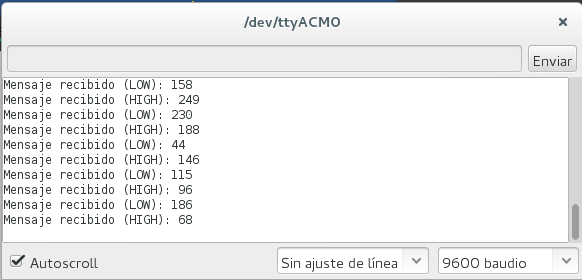
\includegraphics[width=.5\textwidth]{img/Series2RX-consola}
  \caption{Monitor serial del IDE Arduino del ejemplo
    \texttt{Series2\_Rx}.}
  \label{fig:SeriesRxConsola}
\end{figure}

\subsection{Envío de datos periódicos (\emph{Samples Mode})}

Los módulos XBee que se encuentren configurados como
\textsl{end-devices} pueden configurar sus diferentes GPIO de forma
tal que envíen información 

Los módulos XBee ZB tienen la posibilidad de monitorear los canales
analógicos y digitales habilitados. En esta configuración el módulo
puede leer para uso local o transmitir la información relevada a otro
módulo en forma remota. Para esto debe habilitarse el modo
API\cite{s2c-ds}.

En nuestro caso, se configura a uno de los dispositivos considerado
\textsl{end-devices} de forma tal que envíe en forma periódica (cada 2
segundos) los estados de sus diferentes puertos habilitados
(analógicos y digitales). En la Figura \ref{fig:iosample-config} se
muestra el parámetro que define esta funcionalidad de los XBee. Este
módulo es parte de un sistema donde también hay un dispositivo central
(coordinador). Este último recibirá los datos enviados desde los
\textsl{end-devices}. Por esta razón los módulos no tienen la
necesidad de configurar la dirección de destino pues todos los datos
serán enviados al coordinador de la red.

\begin{figure}[h]
  \centering
  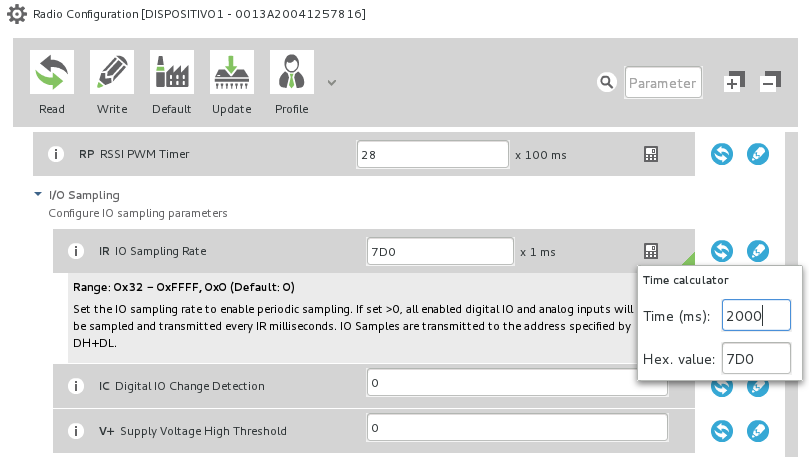
\includegraphics[width=.8\textwidth]{img/ioSampleConfig}
  \caption{Configuración en \textsl{Samples Mode} utilizando la
    aplicación XCTU.}
  \label{fig:iosample-config}
\end{figure}

La librería \texttt{xbee-arduino} dispone de un ejemplo donde la
plataforma arduino está conectado al coordinador de la red ZigBee. El
código \ref{code:iosamples} muestran las principales líneas del ejemplo
\texttt{Series2\_IoSamples}. El ejemplo crea un objeto
\texttt{ZBRxIoSampleResponse} al que se le vinculará  con el paquete
recibido por algún módulo \textsl{end-devices} (línea
\textbf{24}). Los mensajes que recibe el coordinador se presentan en
la consola IDE Arduino identificando a cada uno con su dirección
(líneas \textbf{28-29}). Cada \textsl{frame} incluye la cantidad de
entradas analógicas y digitales habilitadas por parte del
\textsl{end-device} que envía el dato (líneas \textbf{41-56}).

\begin{lstlisting}[basicstyle=\ttfamily\small, language= C++,
  caption={Ejemplo \texttt{Series2\_IoSamples}},label=code:iosamples,
  frame=single]
#include <XBee.h>

XBee xbee = XBee();

ZBRxIoSampleResponse ioSample = ZBRxIoSampleResponse();

XBeeAddress64 test = XBeeAddress64();

void setup() { 
  Serial1.begin(9600);
  xbee.setSerial(Serial1);
  // start soft serial
  Serial.begin(9600);
}

void loop() {
  //attempt to read a packet    
  xbee.readPacket();

  if (xbee.getResponse().isAvailable()) {
    // got something

    if (xbee.getResponse().getApiId() == ZB_IO_SAMPLE_RESPONSE) {
      xbee.getResponse().getZBRxIoSampleResponse(ioSample);

      Serial.print("Received I/O Sample from: ");
      
      Serial.print(ioSample.getRemoteAddress64().getMsb(), HEX);  
      Serial.print(ioSample.getRemoteAddress64().getLsb(), HEX);  
      Serial.println("");
      
      if (ioSample.containsAnalog()) {
        Serial.println("Sample contains analog data");
      }

      if (ioSample.containsDigital()) {
        Serial.println("Sample contains digtal data");
      }      

      // read analog inputs
      for (int i = 0; i <= 4; i++) {
        if (ioSample.isAnalogEnabled(i)) {
          Serial.print("Analog (AI");
          Serial.print(i, DEC);
          Serial.print(") is ");
          Serial.println(ioSample.getAnalog(i), DEC);
        }
      }

      // check digital inputs
      for (int i = 0; i <= 12; i++) {
        if (ioSample.isDigitalEnabled(i)) {
          Serial.print("Digital (DI");
          Serial.print(i, DEC);
          Serial.print(") is ");
          Serial.println(ioSample.isDigitalOn(i), DEC);
        }
      }
      
      // method for printing the entire frame data
      //for (int i = 0; i < xbee.getResponse().getFrameDataLength(); i++) {
      //  Serial.print("byte [");
      //  Serial.print(i, DEC);
      //  Serial.print("] is ");
      //  Serial.println(xbee.getResponse().getFrameData()[i], HEX);
      //}
    } 
    else {
      Serial.print("Expected I/O Sample, but got ");
      Serial.print(xbee.getResponse().getApiId(), HEX);
    }    
  } else if (xbee.getResponse().isError()) {
    Serial.print("Error reading packet.  Error code: ");  
    Serial.println(xbee.getResponse().getErrorCode());
  }
}
\end{lstlisting}  

En la Figura \ref{fig:iosamples} se presenta la consola con la
información proporcionada por el código \ref{code:iosamples}. 
\begin{figure}[h]
  \centering
  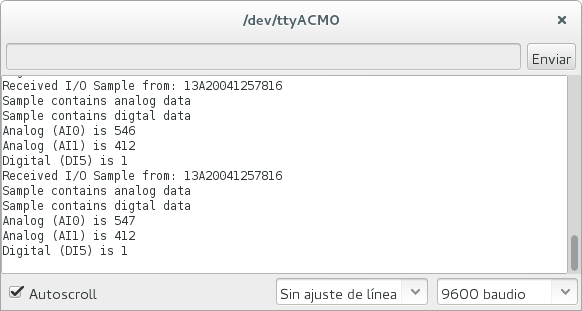
\includegraphics[width=.5\textwidth]{img/iosamples-consola}
  \caption{Monitor serial del IDE Arduino del ejemplo
    \texttt{Series2\_IoSamples}.}
  \label{fig:iosamples}
\end{figure}

\section{Conclusiones}
\label{sec:conc}

Los sistemas en los que requieren la implementación de pequeñas redes
locales inalámbricas se caracterizan por la autonomía de los
dispositivos, el alcance, topología y compromiso entre costo/beneficio
que prestan los potenciales candidatos. En el módulo \emph{Entornos
  Inalámbricos} se propone la utilización de los módulos XBee de Digi
International. Estos módulos implementan el estándar IEEE 802.15.4. Sí
bien existen otros módulos comerciales con menos llegada a un costo
menor\footnote{Por ejemplo, SparkFun Transceiver Breakout:
  \burl{https://www.sparkfun.com/products/691}}, estos no presentan la
garantía y posibilidades en rendimiento que los módulos XBee. En las
pruebas realizadas se comprobó la flexibilidad de su utilización. La
posibilidad de utilizar un \emph{Application Programming Interface}
permite la interacción con otros sistemas embebidos de una manera
mucho más amigable que los comandos AT. En esta línea, las plataformas
Arduino son la forma más directa y sencilla de implementar los módulos
XBee en las diferentes configuraciones disponibles. Como se pudo
leer en las diferentes secciones, se comenzó de básico en interactuar
con el módulo XBee en modo AT (\textsl{transparent mode}) al punto
implementar el API y la automatización del envío de datos de los
módulos XBee al coordinador (unidad central de procesamiento del
sistema). 

Como trabajos futuros podría considerarse la utilización de
plataformas de menor costo que proporcione al usuario una API
flexible. Además sería interesante la disponibilidad de mayores
módulos de forma tal que se puedan asomar problemas en el protocolo
utilizado. Quizá algún emulador de pequeñas redes (PAN) pueda ser
deseable.

\begin{thebibliography}{1}

\bibitem{bilb:PathLoss} Recommendation ITU-R P.1238-8.
\emph{Propagation data and prediction methods
for the planning of indoor
radiocommunication systems and
radio local area networks in the
frequency range 300 MHz to 100 GHz}.
P Series Radiowave propagation. 2015.

\bibitem{s2c-ds}
  Digi International,
  \emph{XBee\textsuperscript{\textregistered{}}/XBee-PRO
    ZigBee\textsuperscript{\textregistered{}} RF Module -- User
    Guide}. 2016.
  
\bibitem{xboard}
  Cika Electrónica SRL.,
  \emph{XBoard [-W]}.
  \burl{http://www.cika.com/soporte/Information/Digi-RF/XBee/XBoard_doc.pdf}.

\bibitem{at-cmds}
  Digi International,
  \emph{Knowledge Base -- The AT Command Set}.
  \burl{http://knowledge.digi.com/articles/Knowledge_Base_Article/The-AT-Command-Set}.

\bibitem{XbeeArduinoGit}
  andrewrapp,
\emph{Arduino library for communicating with XBee radios in API mode},
\burl{https://github.com/andrewrapp/xbee-arduino}.

\bibitem{GalileoDS}
  Intel\textsuperscript{\textregistered{}},
  \emph{Galileo Datasheet}.
  \burl{http://www.intel.com/newsroom/kits/quark/galileo/pdfs/Intel_Galileo_Datasheet.pdf}.

\bibitem{at-cmds}
Digi International,
\emph{Knowledge Base -- The AT Command Set}.
\burl{http://knowledge.digi.com/articles/Knowledge_Base_Article/The-AT-Command-Set}.
\end{thebibliography}

% \appendix{}

% \chapter{Códigos del programa}
% \label{chap:code-prog}

% \lstinputlisting[basicstyle=\scriptsize,title=Código de la función
% \texttt{main.c}]{src/examples/adc_dac/src/adc_dac.c}

% \lstinputlisting[basicstyle=\scriptsize,title=Código del archivo
% \texttt{proyectofinal.oil}]{src/examples/adc_dac/etc/adc_dac.oil}

% \chapter{Esquemáticos del hardware utulizado}
% \label{chap:sch}

% \includepdf[landscape=true,pages=-]{img/Schematic}

\end{document}
